% This is the template Jun uses for project seeds
% jun.allard@uci.edu allardlab.com
\documentclass[onecolumn,11pt]{article}

% --------- required packages ---------
\usepackage{enumerate}
\usepackage{enumitem}
\usepackage{graphicx}
\usepackage[colorlinks,allcolors=black]{hyperref}
\usepackage[font=small]{caption}
\usepackage{siunitx}
\usepackage{times}
\usepackage{titlesec}

\usepackage{titling}
\usepackage{authblk} % must come after titling package loading

% --------- standard packages ---------
%\usepackage{amsfonts}
\usepackage{amsmath}
\usepackage{amssymb}
%\usepackage{array}
%\usepackage{bm}
%\usepackage{color}
%\usepackage{chemarr}
%\usepackage{float}
\usepackage[utf8]{inputenc}
\usepackage{lipsum}
%\usepackage{mathtools}
%\usepackage{multicol}
%\usepackage{multirow}
%\usepackage{pdfsync}
%\usepackage{tocloft}
%\usepackage{verbatim}
%\usepackage{wrapfig}


% --------- packages, less often used ---------
%\usepackage[export]{adjustbox}
%\usepackage{amsopn}
%\usepackage{cancel} % adds strikethrough
%\usepackage{CJK} % Chinese Japanese Korean
%\usepackage{dcolumn} % align columns in a table
%\usepackage{dsfont}
%\usepackage{epsfig}
%\usepackage{epstopdf}
%\usepackage{esint} % integrals
%\usepackage{framed}
%\usepackage{physics} %for \vqty, \dd, \dv
%\usepackage{rotating}
%\usepackage{setspace} % set space between lines
%\usepackage{subcaption}
%\usepackage{tcolorbox}
%\usepackage[normalem]{ulem} % for underlining
% --------- for typesetting code blocks --------
%\usepackage{algorithmic} % for code including Matlab
%\usepackage{listings} % for code including Matlab
%\usepackage[numbered,framed,basicstyle]{matlab-prettifier}




\usepackage{internalsubfigures}




%%%%%%%%%%%%%%%%%%%%%%%%%%%%%%%%%%%%%%%%%%%%%%%%%%%%%%%%%%%%
% page layout
\usepackage[margin=1in]{geometry}

% paragraph layout
\setlength{\parindent}{0pt} % paragraph indent - looks best zero
\setlength{\parskip}{0.8em plus 0.1em minus 0.1em} % paragraph spacing
\setlist[itemize]{itemsep=0.0em,topsep=0em}
\setlist[enumerate]{itemsep=0.0em,topsep=0em}
\titlespacing{\paragraph}{0em}{-0.8em}{1em} % for the /paragraph command

% Bibliography setup
\usepackage[numbers,square,sort&compress]{natbib}
\bibliographystyle{unsrtnat}
%\bibliographystyle{biophysj}

\title{A latex package to label externally-created subfigures}
\author[a]{Jun Allard}
\affil[a]{University of California Irvine}


%%%%%%%%%%%%%%%%%%%%%%%%%%%%%%%%%%%%%%%%%%%%%%%%%%%%%%%
\date{} % leave blank for no date
\begin{document}

\maketitle
%%%%%%%%%%%%%%%%%%%%%%%%%%%%%%%%%%%%%%%%%%%%%%%%%%%%%%%

%\begin{abstract}
%Nothing here yet
%\end{abstract}


\begin{busyfigure}[ht]
        \centering
        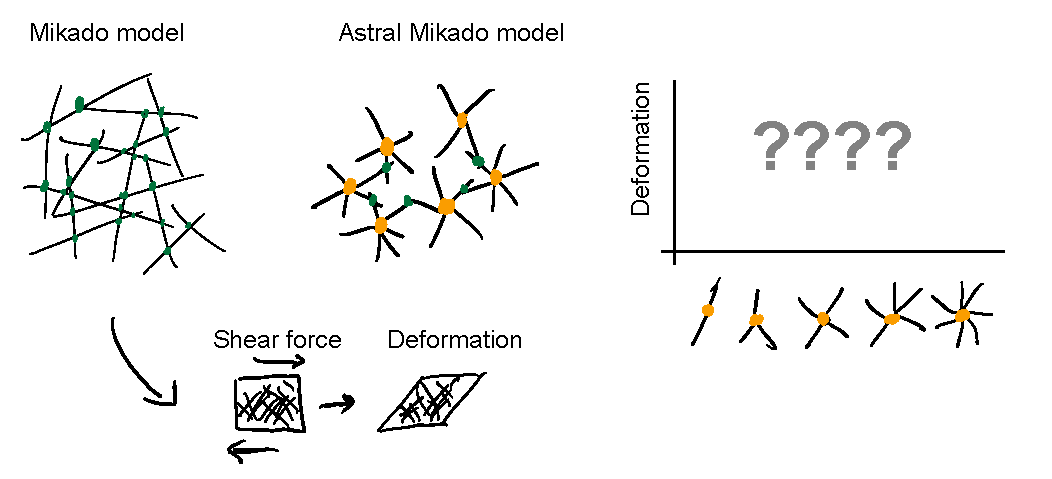
\includegraphics[width=4.5in]{figures/figJeanJacket.pdf}
        \firstsentence{A sentence describing the whole figure.}
        \internalsubfigure{fig:track}{(A) A track that means nothing on its own}
        \internalsubfigure{fig:pcolor}{(B) A pcolor map that also means nothing on its own}
        \majorlabel{fig:omics_conclusion}
\end{busyfigure}

I would like to refer to the main figure Figure~\ref{fig:omics_conclusion}. But this less informative, and instead I should refer to specific panels.

Now, I would like to just refer to the track, Figure~\ref{fig:track}.

Now, I would like to just refer to the colormap, Figure~\ref{fig:pcolor}.


\clearpage

\begin{busyfigure}[ht]
        \centering
        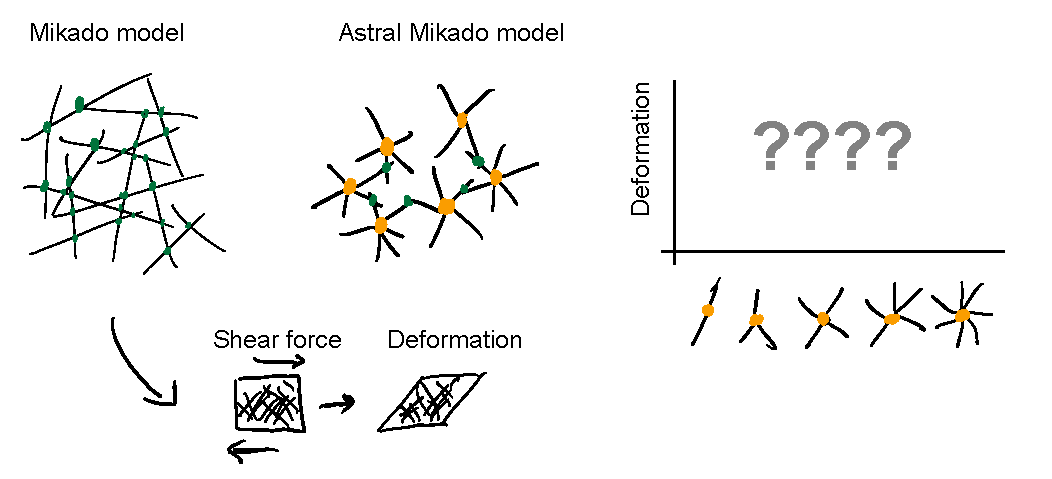
\includegraphics[width=4.5in]{figures/figJeanJacket.pdf}
        \internalsubfigure{fig:gel}{(A) A gel.}
        \internalsubfigure{fig:heatmap}{(B) A heatmap}
        \majorlabel{fig:results_figure}
\end{busyfigure}

I would like to refer to the main figure Figure~\ref{fig:results_figure}. But this less informative, and instead I should refer to specific panels.

Now, I would like to just refer to the gel, Figure~\ref{fig:gel}.

Now, I would like to just refer to the heatmap, Figure~\ref{fig:heatmap}.




\clearpage

\begin{busyfigure}[ht]
        \centering
        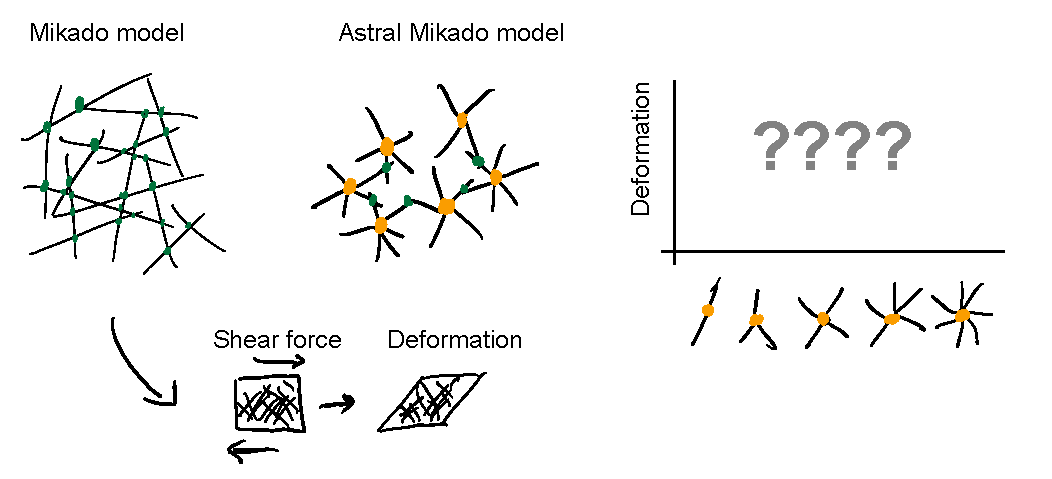
\includegraphics[width=4.5in]{figures/figJeanJacket.pdf}
        \internalsubfigure{fig:schematic}{(A) A schematic to show how all the parts fit together}
        \internalsubfigure{fig:referee_experiment}{(B) A useless and wasteful experiment suggested by Reviewer \#3}
        \majorlabel{fig:final_figure}
\end{busyfigure}

I would like to refer to the main figure Figure~\ref{fig:final_figure}. But this less informative, and instead I should refer to specific panels.

Now, I would like to just refer to the schematic, Figure~\ref{fig:schematic}.

Now, I would like to just refer to the referee-recommended experiment, Figure~\ref{fig:referee_experiment}.


\clearpage

\subsection*{Discussion}

In the discussion, I will discuss all the different subpanels.
For example, the gel in Fig.~\ref{fig:gel}, and the schematic in Fig.~\ref{fig:schematic}.
Or how about the genomic track in Fig.~\ref{fig:track}.


If we move these panels around, all we need to do is change it in the captions (in the \verb|internalsubfigure| lines), and it with automatically change throughout the document! 


\end{document}

